\documentclass[UTF8]{article}

\usepackage{ctex}
\usepackage{marginnote}
\usepackage{listings}
\usepackage{xcolor}
\usepackage[dvipdfm]{graphicx}


\title{插图}
\author{Xmp}
\date{\today}
\begin{document}
\setcounter{tocdepth}{10}
\maketitle
\begin{abstract}
	\begin{quote}
		A picture says more than a thousand words.
		
		\marginnote{---Shakespeare}
		\reversemarginpar
	\end{quote}
\end{abstract}
\tableofcontents


\section{图形概览}
\subsection{图形格式}
对于示意图,我们应该首选矢量格式;包含大量自然色彩的图像 (比如照片)应该选 JPEG;人工点阵图像应该选 PNG。

\subsection{Driver的口味}
\subsubsection{dvips}
\subsubsection{pdflatex}
\subsubsection{dvipdfm(x)}
\subsubsection{xdvipdfmx}

\subsection{图形优化}
矢量图形的一个优点是可以无限缩放,而输出质量不变。图形尺寸对矢量图形而言意义不大。描述矢量图形所需数据较少,所以其文件体积一般也较小。

而点阵图形是以像素 (pixel) 为单位描述、存储的,图形尺寸越大,文件体积就越大。当然影响文件体积的还有色彩深度、压缩算法等因素。

人们一般希望用较小的文件体积获取较好的输出效果,这样就需要优
化图形尺寸和色彩。

\subsubsection{图形尺寸}
点阵图形的信息量取决于像素。图形文件的分辨率只是“建议”缺省输出尺寸,并不影响图形质量。上述操作中裁剪和改尺寸比较实用,改分辨率没有实质意义。改尺寸一般也只能从大改小。如果从小改大的话,插补出来的像素比起原装的还是要差一些。

\subsubsection{色彩深度}
我们一般也只能把图形的色深从高改低,从而减小图形文件和最终文档的体积。

\subsection{图形转换和处理}
命令行界面推荐ImageMagick,
\subsubsection{其他格式转为EPS}
ImageMagick 转换 EPS 的方法如下。如果是 BMP 文件,最好先压缩成JPEG 或 PNG,再转为 EPS,这样生成的 EPS 会比较小。我猜 EPS 的缺省压缩算法可能不如 JPEG 和 PNG。

convert fig.png eps3:fig.eps

另一种方法是用虚拟打印机生成 EPS,它的优点是可以把几乎所有文件“打印”成 EPS。推荐 Bullzip \emph{PDF Printer},它可以把各种文件打印成PS、EPS、PDF、BMP、JPEG、PCX、PNG、TIFF 等格式。用合适的软件打开原始文件,打印到 Bullzip PDF Printer。在 General 标签页把 Format 设置为 EPS,点 Save 按钮就会得到 EPS。

\section{插入图形}
\subsection{范围框}
由于历史原因,latex编译程序不能提取JPEG、PNG等点阵图形的尺寸信息,所以它在处理这些图形文件时需要范围框 (bounding box) 。pdflatex和 xelatex 的用户可以跳过此处,因为它们出现的比较晚,有机会了解这些图形格式。

\subsection{基本命令}
使用graphics和graphicx宏包,插图命令基本用法如下:
\lstset
{
numbers=left, 
numberstyle= \tiny, 
keywordstyle= \color{ blue!70},
commentstyle= \color{red!50!green!50!blue!50}, 
frame=shadowbox, % 阴影效果
rulesepcolor= \color{ red!20!green!20!blue!20} ,
escapeinside=``, % 英文分号中可写入中文
xleftmargin=2em,xrightmargin=2em, aboveskip=1em,
framexleftmargin=2em
}
\begin{lstlisting}
	\usepackage[dvipdfm]{graphicx}
	\includegraphics[bb=0 0 300 200]{fig.png}
\end{lstlisting}

\subsection{图形操作}
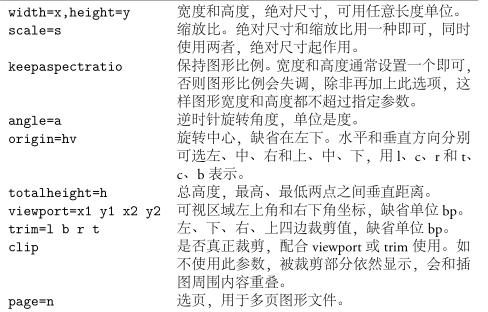
\includegraphics[scale=1.0]{GraphicalOperation.png}






















\end{document}